% !TEX root = main.tex

% TODO:
%   * Acronym to be covered: \sqrt{s}, $pp$
%   * Make a reference to post-run-I appendix
% REMARK:
% . * LHC, CMS are both defined in this section

\clearpage
\section{Experimental Apparatus}
\label{sec:ExperimentalAppratus}
% http://www.lhc-closer.es/taking_a_closer_look_at_lhc/1.lhc_parameters
% https://home.cern/resources/faqs/facts-and-figures-about-lhc

	\subsection{Large Hadron Collider(LHC)}
	\label{ssec:ExpApp_LHC}

	\subsection{Compact Muon Solenoid(CMS) Detector}
	\label{ssec:ExpApp_CMS}

		The CMS use the right-handed system, the x-axis point to the center of LHC, y-axis point up and orthogonal to the ground, and z-axis is along with anti-clockwise beam direction.

		\subsubsection{Magnetic configuration}
		\label{sssec:ExpApp_magnetic}


		\subsubsection{Tracking system}
		\label{sssec:ExpApp_tracking}

			The CMS tracker's schematic drawing is shown below in Fig.\ref{PhysObj:fig:tracker} from reference\cite{Chatrchyan:2014fea} where $\textbf{strip tracker}$ with small silicon tracker within. 

			\begin{figure}[H]
			\centering{}
		    	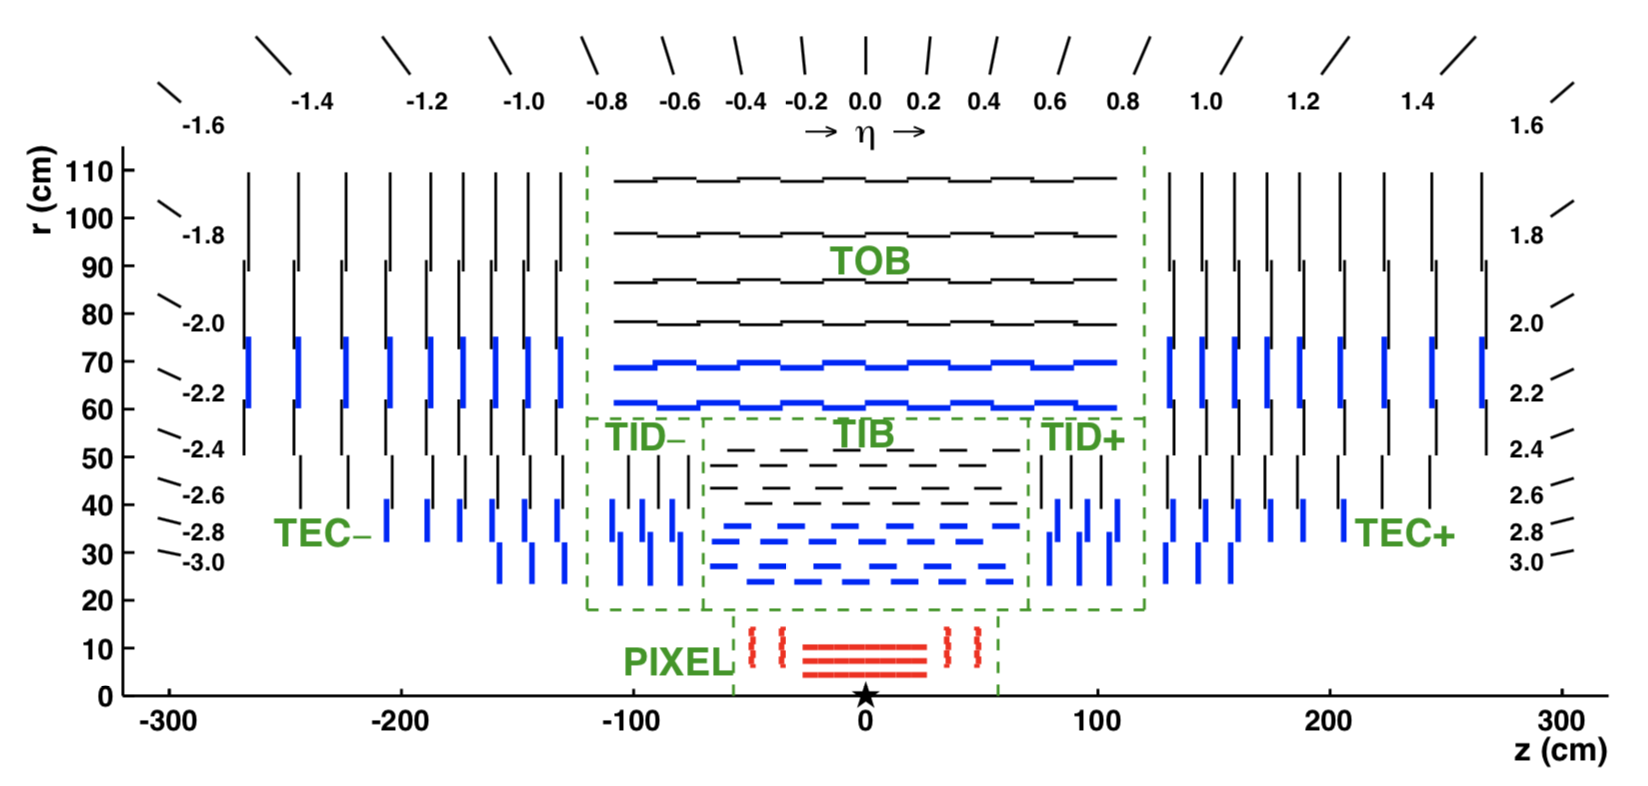
\includegraphics[width=0.85\textwidth]{Figures/ExpApparatus/tracker.png}\\
			\caption{The drawing of the CMS inner tracking system\cite{Chatrchyan:2014fea}}
			\label{PhysObj:fig:tracker}
			\end{figure}
			\FloatBarrier

			Futhermore, the tracker is immersed in magnetic field from CMS solenoid. There are four subsystem in it and they are completed by endcaps(|pseudorapidity $\eta | < 2.5$) on either sides of barrels. The four subsystems are the $\textbf{Tracker Inner Barrel (TIB)}$, the $\textbf{Tracker Inner Disk (TID)}$, the $\textbf{Tracker Outer Barrel(TOB)}$, and the $\textbf{Tracker EndCaps(TEC)}$. There are slices of silicons in these tracking subsystems, and the detail of thickness, position and layers would be found in reference\cite{Chatrchyan:2014fea}. Also, the summary of the principal characteristics of the various tracker subsystems from \cite{Chatrchyan:2014fea} is attached below:
			
			\begin{figure}[H]
			\centering{}
		    	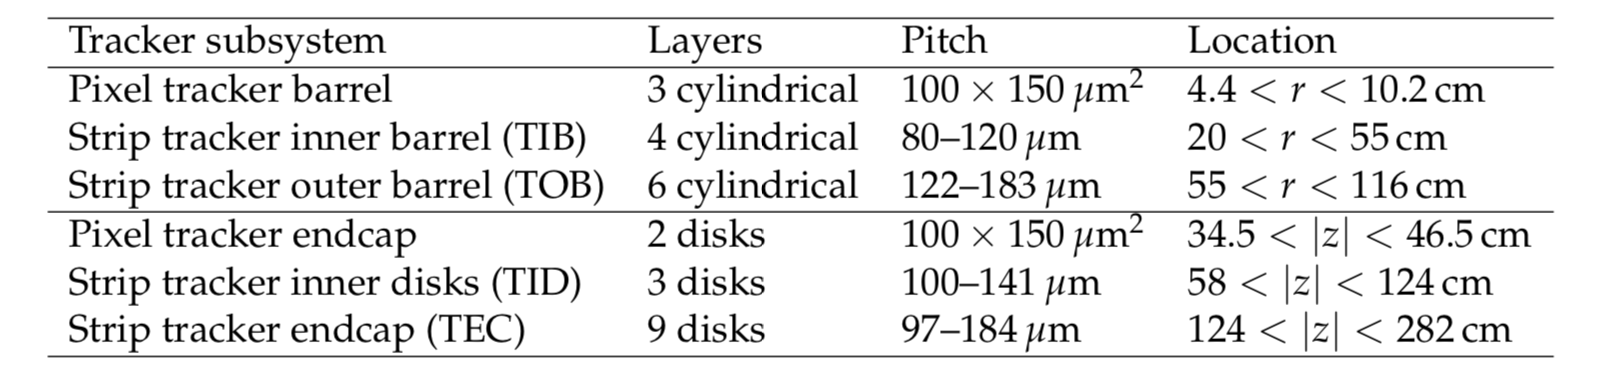
\includegraphics[width=0.85\textwidth]{Figures/ExpApparatus/summary_subtracker.png}\\
			\caption{Summary of the principal characteristics of the various tracker subsystems\cite{Chatrchyan:2014fea}}
			\label{PhysObj:fig:tracker_sum}
			\end{figure}




